% This version of CVPR template is provided by Ming-Ming Cheng.
% Please leave an issue if you found a bug:
% https://github.com/MCG-NKU/CVPR_Template.

%\documentclass[review]{cvpr}
\documentclass[final]{cvpr}

\usepackage{times}
\usepackage{epsfig}
\usepackage{graphicx}
\usepackage{amsmath}
\usepackage{amssymb}

% Include other packages here, before hyperref.

% If you comment hyperref and then uncomment it, you should delete
% egpaper.aux before re-running latex.  (Or just hit 'q' on the first latex
% run, let it finish, and you should be clear).
\usepackage[pagebackref=true,breaklinks=true,colorlinks,bookmarks=false]{hyperref}


\def\cvprPaperID{****} % *** Enter the CVPR Paper ID here
\def\confYear{CVPR 2021}
%\setcounter{page}{4321} % For final version only


\begin{document}

%%%%%%%%% TITLE
\title{Exploring Conditional Invertible Neural Networks \\}

\author{
Final Project for the course Computer Vision: 3D Reconstruction\\\\
Damjan Kalsan, David Scheid, Sebastian Stricker\\
Heidelberg University, WS2021/22\\
}

\maketitle


%%%%%%%%% ABSTRACT
\begin{abstract}
   In the following we document our experiments with the conditional invertible neural network (cINN) architecture as proposed by \cite{main_paper_CINN}.
   In the first part, the concept is illustrated on a simple toy example to provide a more intuitive understanding of the image generation and style transfer process.
   The second part focuses on the application on new data. We chose FashionMNIST \cite{fashion_mnist} as a simple yet diverse dataset and show results and difficulties with image generation and style transfer.
   We build our models using the FrEIA framework \cite{freia}
\end{abstract}

%%%%%%%%% BODY TEXT
\section{Introduction}
In usual classification tasks with neural networks, a network is trained to predict a class label, a one hot encoded vector $y$, given an input vector $x$. This can be represented as $f(x; \theta) = y$, with $\theta$ being the network weights.

In contrast to this, cINNs are provided with this information by a conditioning vector $c$ during the forward pass already. The resulting output or latent vector $z$ necessarily matches the input in dimension to preserve invertibility of the network. Figure \ref{fig:cINN_concept} illustrates the concept.

This key property of invertibility allows for the inverse mapping  $z \rightarrow x$. Equation \ref{eq:cINN} captures this. It is achieved by constructing the network as a concatenation of coupling blocks as introduced by \cite{RealNVP}.
For the technical details, we refer to the original publications.

\begin{equation} \label{eq:cINN}
\begin{split}
		f(x;c;\theta) 		= z \\
		f^{-1}(z;c;\theta) 	= x
\end{split}
\end{equation}

For the models discussed in this work $c$ can be seen as equivalent to the ground truth one-hot encoding $y$. This is not necessary the case, however, as demonstrated by more complex image coloration architectures \cite{main_paper_CINN}.

\begin{figure}[t]
	\begin{center}
		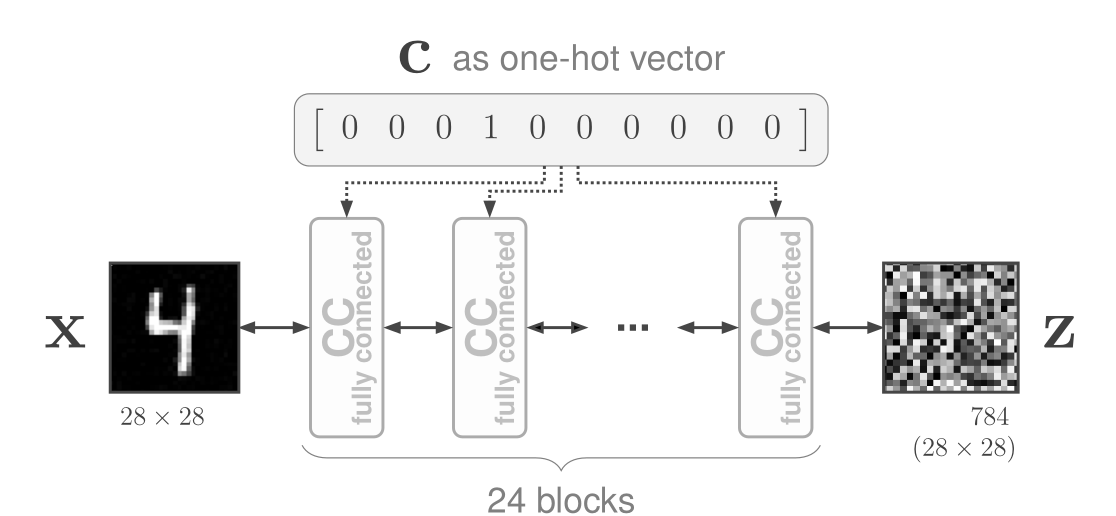
\includegraphics[width=0.8\linewidth]{./figs/cINN_MNIST_model.png}
	\end{center}
	\caption{Illustration of cINN Architecture for MNIST digit classification. Class labels are concatenated to the intermediate input in each coupling layer. Taken from \cite{main_paper_CINN}}
	\label{fig:cINN_concept}
\end{figure}

\subsection{Interpreting the latent vector}
As class information is provided as input for each coupling block, this information is inherently not part of the networks output $z$. It raises the question of what information $z$ is supposed to contain.

Assume for training data $X$, $Z = \{f(x_i;c;\theta) \,|\, x_i \in X\}$ is the set of all $z$ that are an output of the network. The training enforces $Z$ to take the form of a probability distribution $p_Z(z)$. For simplicity, we assume it to be the standard normal. The training Loss is then a maximum likelihood calculation, meaning the inverse pass returns the most likely $x$ given a $z$ and the weights are adjusted for disagreement.
For technical details, we again refer to the original publication \cite{main_paper_CINN}.

As will be shown in section \ref{toy}, interpreting the individual dimensions in the latent space is not trivial. But seen as a whole, $z$ has to capture all the features that make up our input in order to ensure the map $z \rightarrow x $ holds, while maintaining the property that the complete set $Z$ forms a probability distribution. 

\subsection{Image generation and style transfer}
$Z$ is a finite set, but the probability distribution enforced on the set is a continuous function. Therefore, it is possible to sample from the distribution to obtain a $z' \notin Z$. Running the network in reverse results in $f^{-1}(z';c;\theta) = x'$. $x'$ is then a result, that has not been generated before. 

For style transfer, a $z$ is obtained form an arbitrary $x$ via the network $f(x;c_x;\theta) = z$. Setting $c' \neq c_x$, the style of $x$ can be mapped to all other class labels via $f(z;c';\theta)$.

\section{Toy example}\label{toy}
In the following, a simple example using 4 gaussian distributions is used to illustrate and explore properties of the cINN mappings described in the Introduction.

The model used consists of 8 AllInOne coupling blocks, described in the framework \cite{freia}. As a subnet for each block, a fully connected network with 2 hidden layers and 256 nodes each is employed.

\begin{figure*}[t]
	\begin{center}
		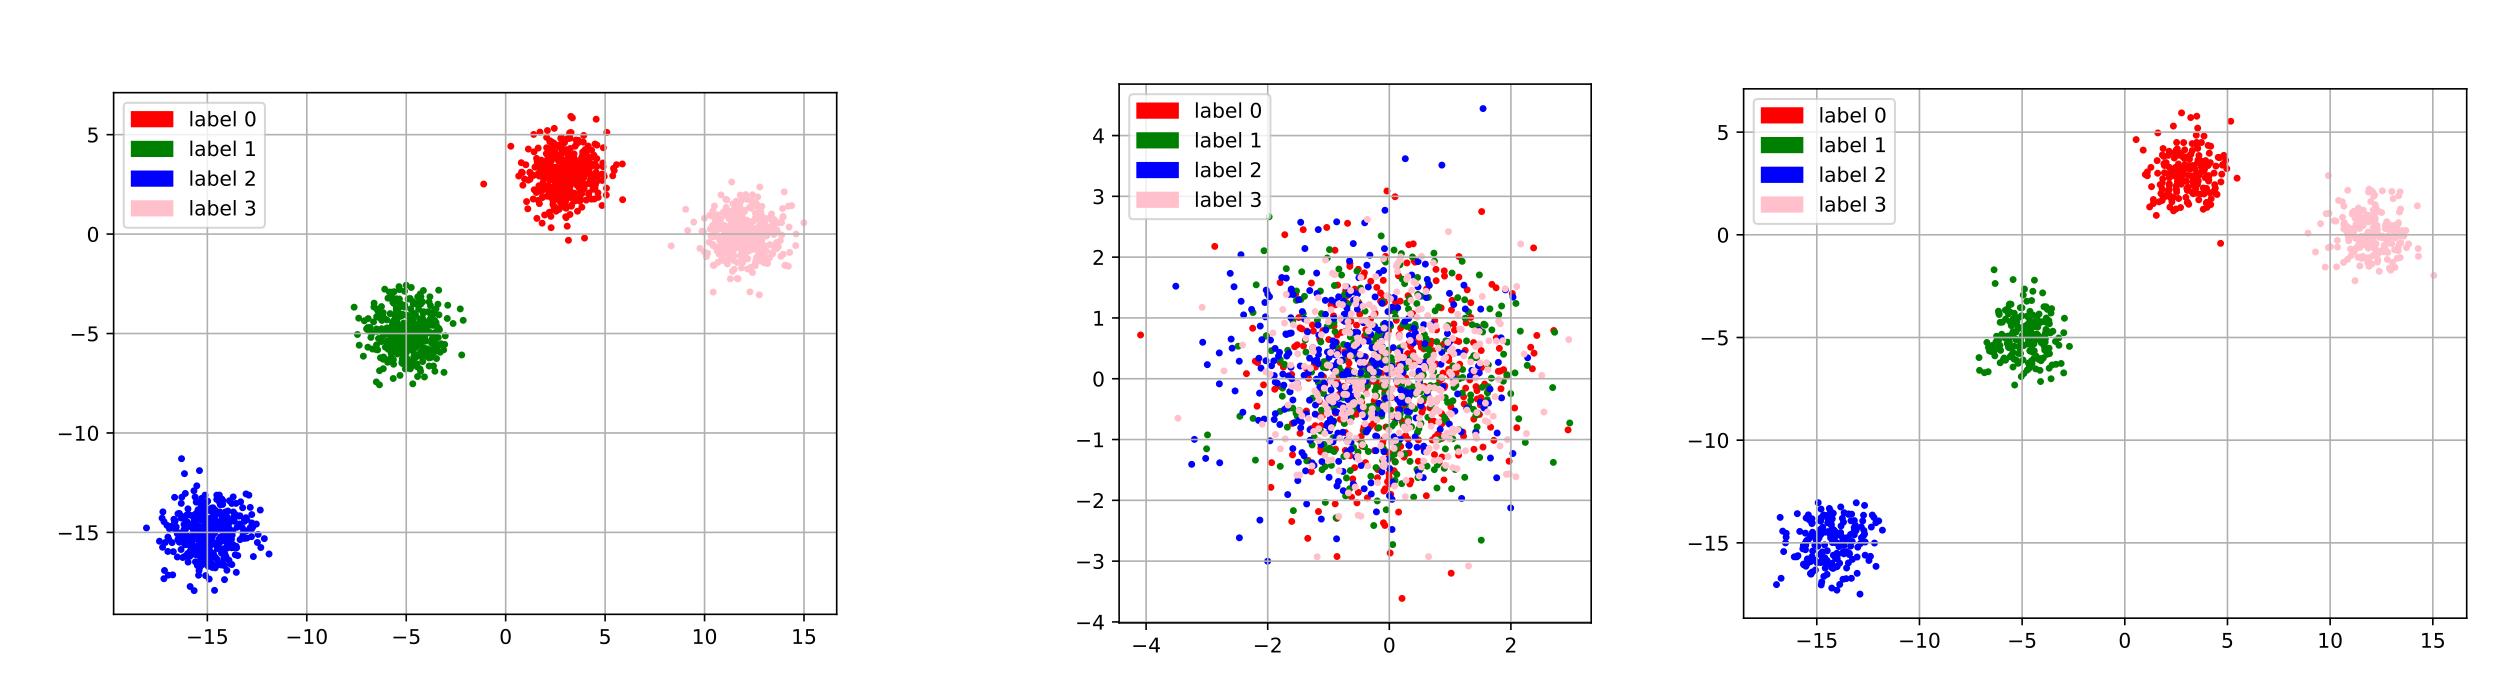
\includegraphics[width=1.0\linewidth]{./figs/toy/no_style/combined.png}
	\end{center}
	\caption{(left) Input data. (middle) Latent space after training. (right) Data generated with newly sampled z values.}
	\label{fig:toy_generation}
\end{figure*}

\subsection{Sample Generation}\label{sec:toy_sample}
Figure \ref{fig:toy_generation} depicts the process of image generation. 

The left plot shows the input data. Each distribution contains 800 samples. Labels used for conditioning indicate which distribution a point originates from and are color coded in the plots to visually differentiate between them.
Positions of samples form the respective input vector $x = (\hat{x}, \hat{y})$

The middle image depicts the latent space $Z$ after training. Visibly, the values form a normal distribution as enforced by training. Further, the values are not separated by label. Clearly no classification information is stored in the latent space.

The right image depicts the result of data generation. For each label, 200 values from a two dimensional normal distribution were drawn and passed through the inverse network.
As can be seen, the data was successfully classified even though the $z$ values used were not part of the training process.

\subsection{style transfer}
To make matters more interesting, each sample was enhanced with an attribute from the set $S = \{0.0, 1.0, 2.0\}$. The input vector is then formed by $x = (\hat{x}, \hat{y}, s)$, with $s \in S$ chosen randomly for each sample.

After training, 5 samples from label 0 distribution were evaluated resulting in $Z'=\{z_1, z_2, z_3, z_4, z_5\}$. For all labels, these $z$ samples were then passed through the inverse network. 
The results are depicted in Figure \ref{fig:toy_style}. The plot to the left shows the input distributions and the one to the right the results after style transfer. 
Attribute value s is indicated by shape and was rounded to the nearest integer after the inverse pass.

As can be seen, the samples with label 1,2,3 have successfully received the shapes from the samples with label 0. This result was consistent over many attempts. 

Position transfer, on the other hand, does not seem to work consistently. In the example depicted here, apart from small deviations, samples in label 0 and 1 seem to have been assigned equivalent positions. Samples in label 2 and 3 have been rotated counterclockwise by 90°.
Depending on training success and chance, results on position transfer range from fully consistent to not correlated at all.

\begin{figure*}[t]
	\begin{center}
		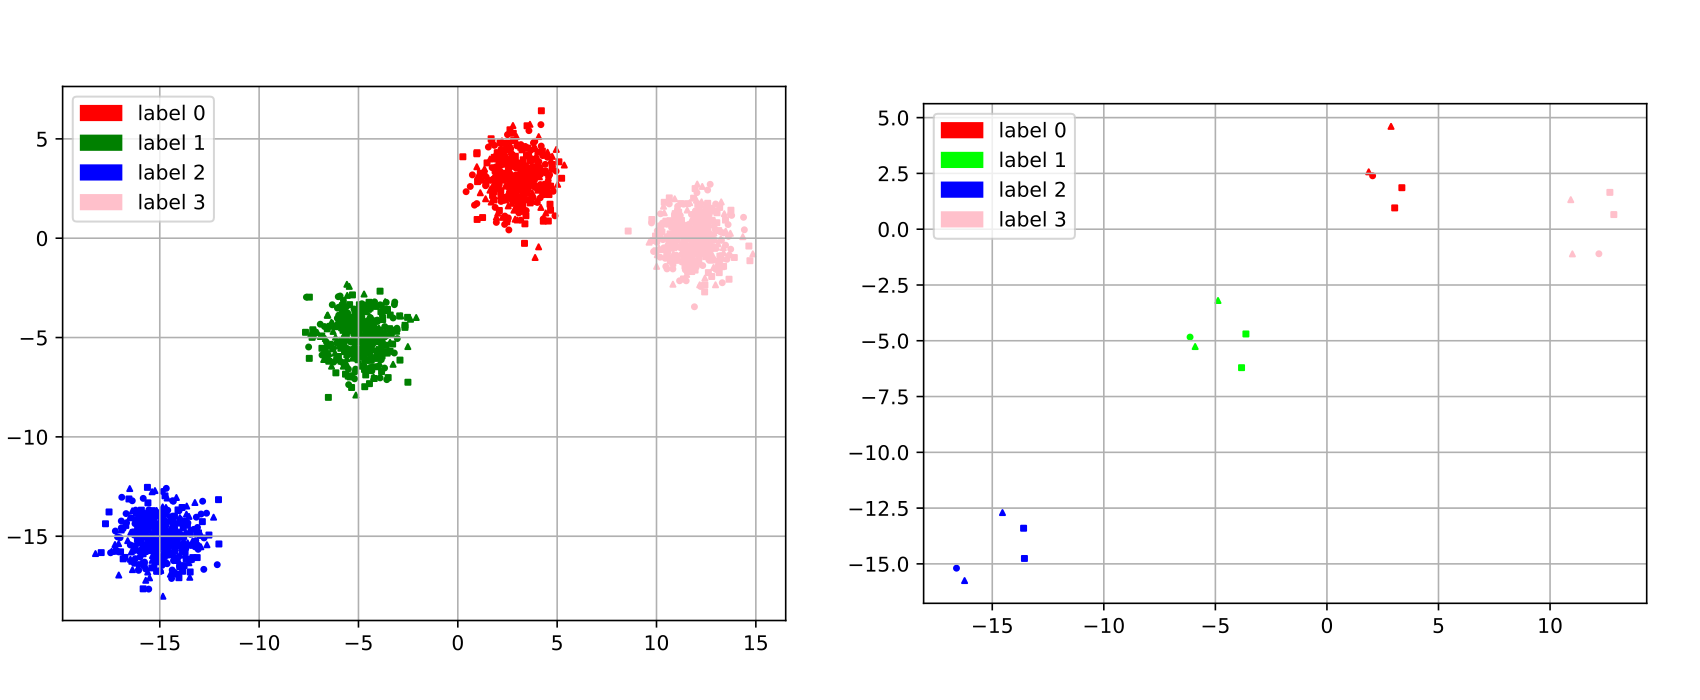
\includegraphics[width=1.0\linewidth]{./figs/toy/with_style/combined_style_transfer.png}
	\end{center}
	\caption{(left) Input data. Attribute $s$ is plotted as corresponding shape \{circle, square, triangle\} (right) Successful style transfer of label 0 to all labels.}
	\label{fig:toy_style}
\end{figure*}

\subsection{Attribute enhanced latent space}
To close the section on the toy example, it is shown that dimensions in the latent space do not necessarily capture information independent from each other. 

Similar to the sample generation as described in section \ref{sec:toy_sample}, 200 $z$ vectors were sampled from the three dimensional normal distribution.
Dimensions were then searched for correlation with attribute information $s$. The corresponding dimension differs for each training run. 

In the network analysed, the second dimension contained the highest degree of information. For each sample a constant value $c$ replaced the corresponding value $z = (z^1, z^2, z^3) \rightarrow (z^1, c, z^3)$.

Figure \ref{fig:latent} shows the results for $c = \{-2.0, 0.0, 2.0\}$. As can be observed, the samples do all receive the same attribute, however, the positions are in no example as clear as in the initial distributions.
It can be concluded, that the latent space dimensions are not easily separable in this example.

\begin{figure*}[t]
	\begin{center}
		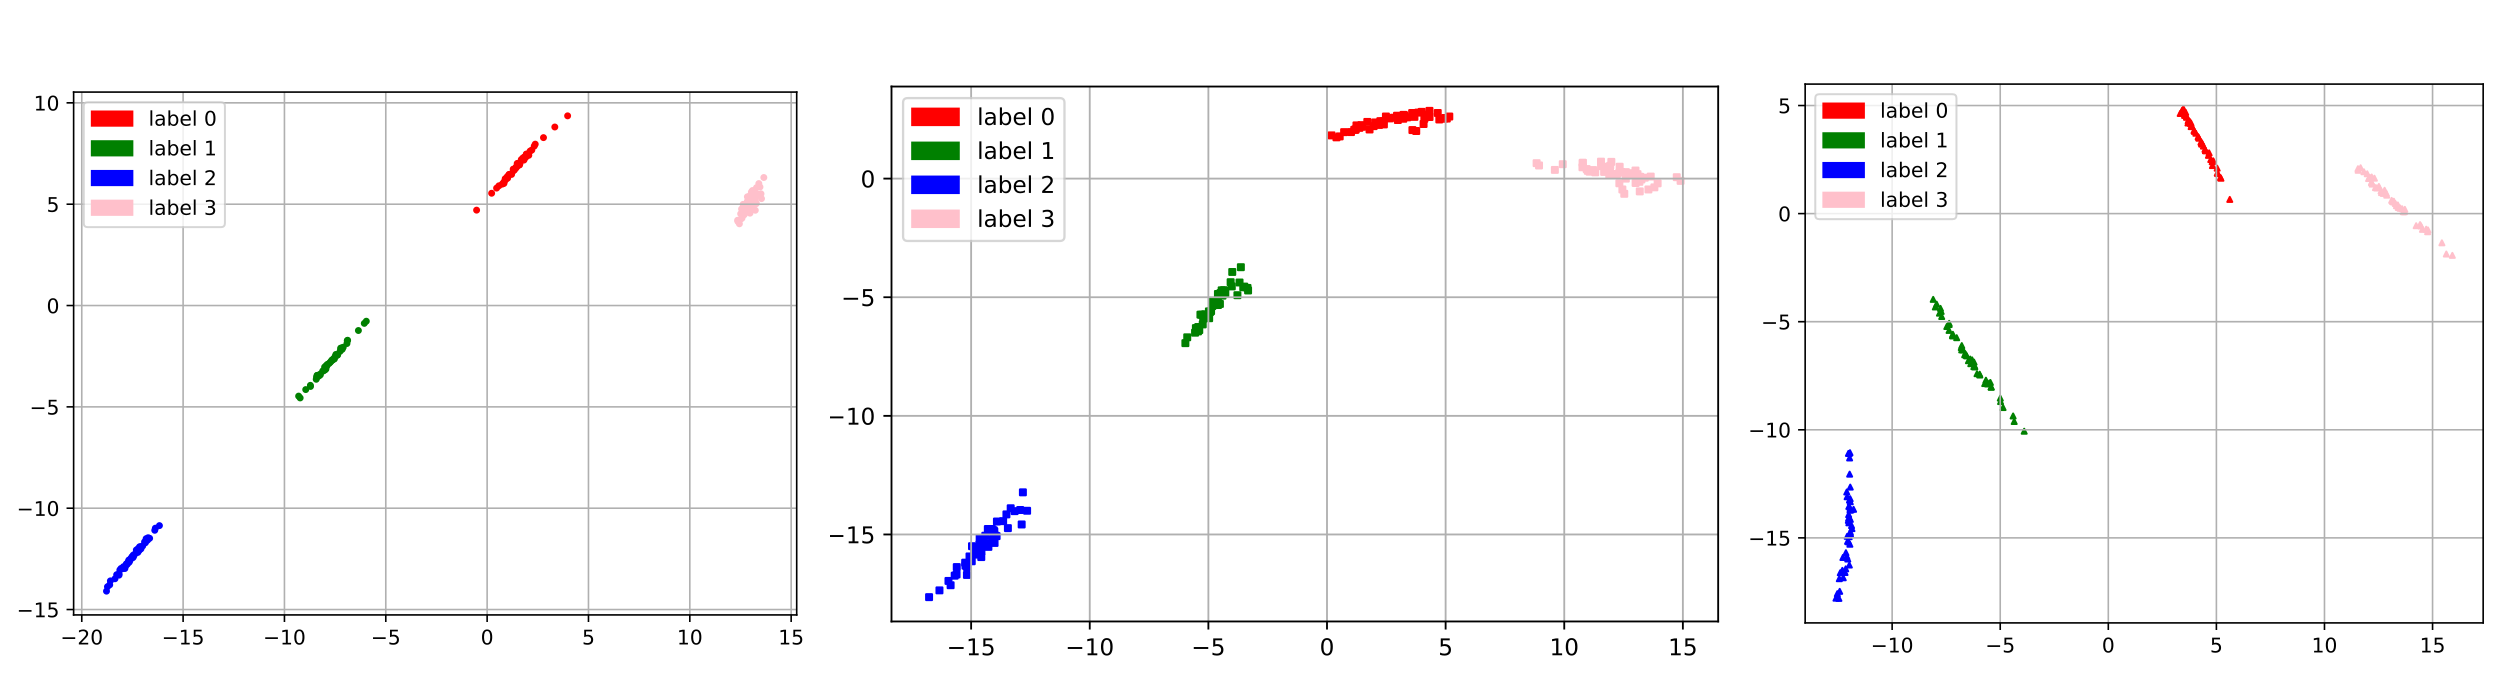
\includegraphics[width=1.0\linewidth]{./figs/toy/with_style/combined_reverse_sample.png}
	\end{center}
	\caption{(left) $c = -2.0 \Rightarrow s = 0.0$ (circle). (middle) $c = 0.0 \Rightarrow s = 1.0$ (square). (right) $c = 2.0 \Rightarrow s = 2.0$ (circle).}
	\label{fig:latent}
\end{figure*}






{\small
\bibliographystyle{ieee_fullname}
\bibliography{bibliography}
}

\end{document}
